\section{Python Interpreter}

In order to obtain a thorough understanding of compilers, it is necessary to learn
how interpreters work and operate. By drawing this comparison between compilers and
interpreters it is possible to appreciate the benefits, but also acknowledge the
disadvantages both systems entail. By example of Python this section walks through
the design of an interpreter at a high-level which will be rounded up with a subsequent
evaluation in the next chapter.

At the highest level, the Python interpreter consists of two components: a compiler
that produces platform-independent bytecode, and the PVM (Python Virtual Machine)
which interprets and subsequentially executes the program. In addition to that,
the PVM accepts custom user input as well as pre-compiled library modules before
it goes over to execute the program.

\begin{figure}[ht]
    \centering
    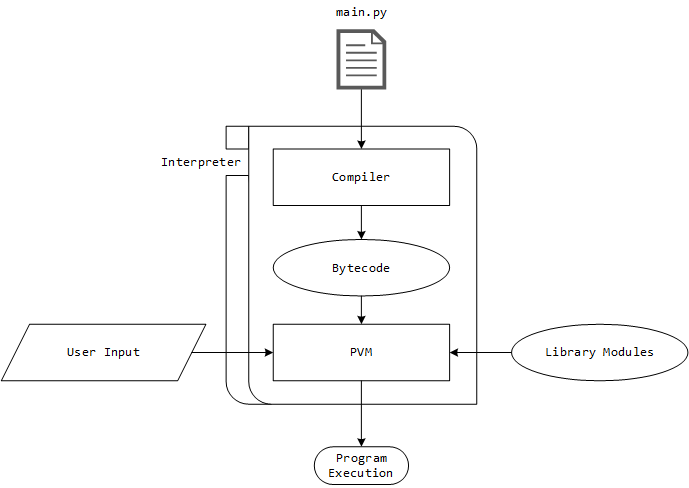
\includegraphics[width=0.7\textwidth]{images/BasicPythonArchitecture.png}
\end{figure}

At the second-highest level, the Python interpreter can be divided into three major
components: Parser, Compiler and PVM. Inside the parser, the scanner removes all
comments, white spaces, etc. to create a token stream that is passed on to the
Python parser, which in turn creates a parse tree. Note that the parse tree does
not contain any automated or symbolic connection between grammar specification and
the individual nodes in the parse tree. This parse tree is converted into an abstract
syntax tree by the AST converter. The AST is the highest-level representation of
the program structure where each AST node contains information about statements,
expressions, and several other specialized types like list comprehension and exception
handlers. The code generator takes the AST and translates it into a CFG (Control
Flow Graph) that can be thought of as an IR (intermediate representation) within
the blocks.

\begin{figure}[h]
    \centering
    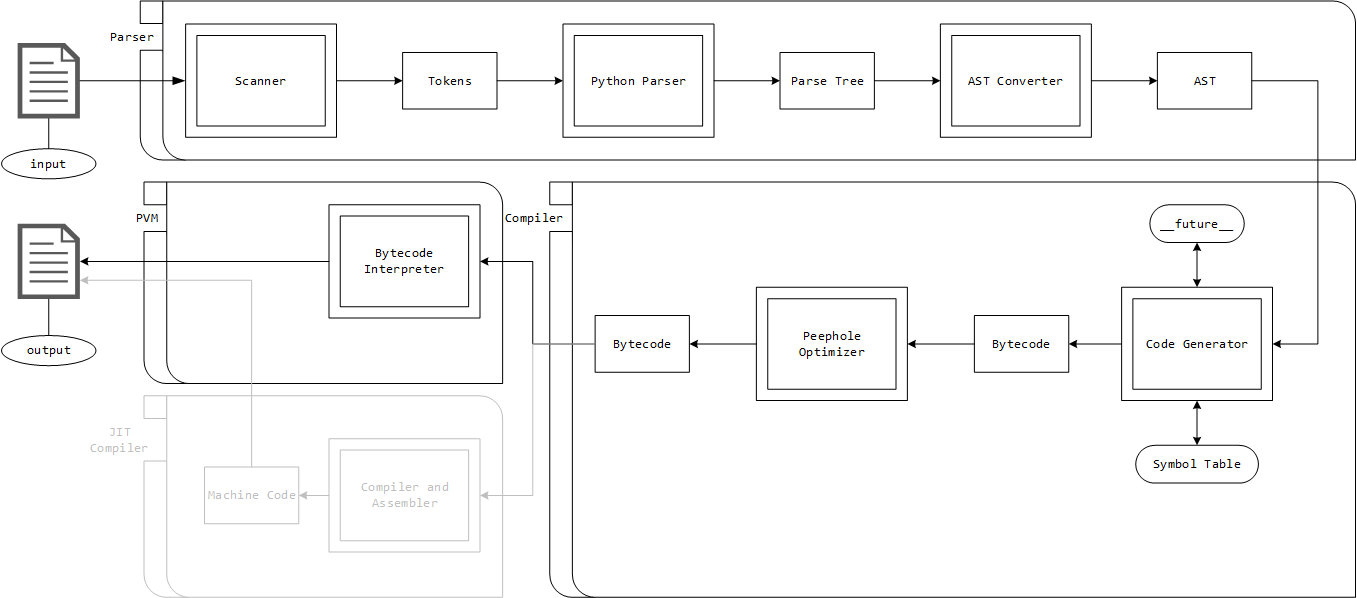
\includegraphics[width=1\textwidth]{images/PythonArchitecture.png}
\end{figure}

Basic blocks themselves are a block of IR with one entry point (that is the target
of something with the potential of changing the control flow) and possibly multiple
exit points which can change the flow of the program by using jumps or return
statements. Bytecode is generated directly from the CFG by doing a post-order
depth-first search on the CFG following the edges. After that the bytecode goes
through the peephole optimizer before it enters the PVM. From then on, there are
two possible paths that can be taken before the program execution takes place:

\begin{enumerate}
    \item CPython is the reference implementation of the Python programming language
    which utilizes a bytecode interpreter to trigger the program execution.
    \item Alternative language implementations (such as Numba\footnote{Numba is
    an open-source JIT compiler that translates a subset of Python and NumPy code
    into machine code by using the LLVM compiler library.}, PyPy\footnote{Uses an
    interpreter written in RPython and a JIT compiler to translate the source code
    into machine code instructions.}, or IronPython\footnote{Targets Microsoft's
    .NET framework and uses its JIT compiler to improve the program execution time.
    This implementation also removes the python's built-in GIL (Global Interpreter
    Lock).}, employ a JIT compiler to reduce the overhead that is caused by the
    interpreter by translating the bytecode into machine code instructions which
    often improves the performance of the program significantly.
\end{enumerate}

In CPython, memory is pooled in a single location for easy allocation and removal.
Because memory allocation for all needed memory in the compiler registers that memory
with the arena, a single call to free the arena is all that is needed to completely
free all memory used by the compiler \autocite{python2021}. Python stores all data
structures in a private heap which is managed by Python's memory manager and can
be divided into four distinct types \autocite{zehra2020}:

\begin{enumerate}
    \item \textbf{Heap} is a collection of all memory chunks managed by Python.
    \item \textbf{Arenas} are the largest chunks of memory which have a fixed
    size of 256 KB each. Python requests them from the system and they are the
    object that make up the heap.
    \item \textbf{Pools} are chunks of memory stored as arrays that make up the
    arenas that measure 4 KB each.
    \item \textbf{Blocks} have a specific format based on their data types. Python
    objects are stored in blocks. For example, an integer takes up more space than
    a character. For sake of efficiency, a different block size is used to store
    that object. 
\end{enumerate}

In summary, memory allocation and deallocation are handled by the GC (Garbage
Collector) run by the PVM. Objects that go out of scope become eligible for
release by the GC. Hence, virtually most of the time manual memory management
can be completely ignored by the programmer.
